% Presentación del avance (Beamer 16:9). Compilar dos veces: pdflatex presentacion_avance.tex
\documentclass[aspectratio=169,11pt]{beamer}
\usepackage[utf8]{inputenc}
\usepackage[T1]{fontenc}
\IfFileExists{spanish.ldf}{\usepackage[spanish,es-noshorthands]{babel}}{}
\usepackage{lmodern}
\usepackage{booktabs}
\usepackage{tabularx}
\usepackage{array}
\usepackage{tikz}
\usetikzlibrary{arrows.meta,positioning}
\graphicspath{{figuras/}{../avance_latex/figuras/}}

% ---------- estilo ----------
\definecolor{azul}{HTML}{0B3D5C}
\definecolor{azulc}{HTML}{0B5D8F}
\definecolor{acento}{HTML}{D4145A}
\definecolor{ok}{HTML}{1B7F4B}
\definecolor{naranja}{HTML}{E8710A}
\definecolor{gris}{HTML}{5B6770}
\usetheme{default}
\setbeamercolor{frametitle}{fg=white,bg=azul}
\setbeamercolor{title}{fg=white}
\setbeamercolor{structure}{fg=azulc}
\setbeamercolor{alerted text}{fg=acento}
\setbeamercolor{block title}{fg=white,bg=azulc}
\setbeamercolor{block body}{bg=azulc!7}
\setbeamercolor{block title alerted}{fg=white,bg=acento}
\setbeamercolor{block body alerted}{bg=acento!7}
\setbeamercolor{block title example}{fg=white,bg=ok}
\setbeamercolor{block body example}{bg=ok!7}
\setbeamertemplate{navigation symbols}{}
\setbeamertemplate{itemize items}[circle]
\setbeamerfont{frametitle}{size=\large,series=\bfseries}
\setbeamertemplate{frametitle}{\nointerlineskip\begin{beamercolorbox}[wd=\paperwidth,ht=2.6ex,dp=1.3ex,leftskip=1em]{frametitle}\insertframetitle\end{beamercolorbox}}
\setbeamertemplate{footline}{\hbox{\begin{beamercolorbox}[wd=\paperwidth,ht=2.4ex,dp=1ex,leftskip=1em,rightskip=1em]{}%
  \color{gris}\tiny Inundaciones por El Niño · Tumbes y Piura · PEU-CD INEI\hfill\insertframenumber/\inserttotalframenumber\end{beamercolorbox}}}
\newcommand{\cifra}[2]{\begin{minipage}[t]{0.23\textwidth}\centering{\Large\bfseries\color{azul}#1}\\[1pt]{\scriptsize #2}\end{minipage}}

\title{Exposición potencial a inundaciones asociadas a El Niño\\en Tumbes y Piura}
\subtitle{Avance del proyecto integrador · PEU Ciencia de Datos (INEI)}
\author{Christopher · Maykol · Marcia · Luz Ángela}
\date{4 de noviembre de 2026}

\begin{document}

% ---------- portada ----------
{\setbeamertemplate{footline}{}
\begin{frame}
\begin{tikzpicture}[remember picture,overlay]
  \fill[azul] (current page.north west) rectangle ([yshift=-5.3cm]current page.north east);
  \node[anchor=north west,text width=13.5cm,text=white] at ([xshift=1cm,yshift=-1.1cm]current page.north west)
    {{\LARGE\bfseries Exposición potencial a inundaciones asociadas a El Niño en Tumbes y Piura}\\[8pt]
     {\large Avance del proyecto integrador · PEU Ciencia de Datos (INEI)}};
  \node[anchor=north west,text width=13.5cm] at ([xshift=1cm,yshift=-6.0cm]current page.north west)
    {\large Christopher · Maykol · Marcia · Luz Ángela\\[4pt]
     \normalsize 4 de noviembre de 2026\\[10pt]
     \small\color{gris} Tablero: \texttt{marciashapiama.github.io/iapn-inei}\quad Código: \texttt{github.com/MarciaShapiama/iapn-inei}};
\end{tikzpicture}
\end{frame}}

\begin{frame}{Contenido}
\begin{columns}[T]
\column{0.48\textwidth}
\begin{enumerate}
\item Problema y pregunta
\item Datos y arquitectura
\item Auditoría: qué corregimos
\item Resultados del piloto
\item El tablero
\end{enumerate}
\column{0.48\textwidth}
\begin{enumerate}\setcounter{enumi}{5}
\item ¿Funcionó? Validación
\item Machine learning
\item Aporte al INEI y políticas
\item Viabilidad de expansión
\item Próximos pasos
\end{enumerate}
\end{columns}
\end{frame}

% ---------- 1 ----------
\section{Problema}
\begin{frame}{1. Problema y pregunta de investigación}
\begin{columns}[T]
\column{0.55\textwidth}
\begin{block}{Problema}
Piura y Tumbes sufren inundaciones recurrentes con El Niño (1983, 1998, 2017) y con eventos como el ciclón Yaku (2023). No existe en un solo lugar una cifra \textbf{por distrito}, reproducible y con fuente, de quién y qué queda expuesto.
\end{block}
\begin{block}{Pregunta}
¿Cuánta población, cuántas edificaciones, colegios y establecimientos de salud están \textbf{potencialmente expuestos} y qué distritos deben revisarse primero?
\end{block}
\column{0.42\textwidth}
\begin{alertblock}{Reglas de lectura}
\small
\begin{itemize}
\item «Expuesto» $\neq$ afectado ni damnificado.
\item Un escenario de 1 en 100 años no anuncia una inundación este año.
\item No emitimos alertas: son de SENAMHI, ENFEN e INDECI.
\end{itemize}
\end{alertblock}
\small\textbf{Alcance:} piloto en 76 distritos (UBIGEO). La expansión es una fase posterior.
\end{columns}
\end{frame}

% ---------- 2 ----------
\section{Datos}
\begin{frame}{2. Datos que usamos (todos abiertos y gratuitos)}
\scriptsize
\renewcommand{\arraystretch}{1.12}
\begin{tabularx}{\textwidth}{>{\raggedright\arraybackslash}p{3.8cm}>{\raggedright\arraybackslash}X>{\raggedright\arraybackslash}p{1.8cm}>{\raggedright\arraybackslash}p{2.4cm}}\toprule
\textbf{Tema} & \textbf{Fuente} & \textbf{Resolución} & \textbf{Naturaleza}\\\midrule
Peligro fluvial 1/10 y 1/100 años & JRC CEMS-GloFAS v2 & 90 m & escenario\\
Agua observada 2017, 2023 y reciente & Sentinel-1 (Copernicus) vía Planetary Computer & 55 m & observado (derivado)\\
Población & WorldPop 2026 & 100 m & modelado\\
Edificaciones & Google Open Buildings v3 & huella & observado (ML)\\
Colegios / Salud & OpenStreetMap / RENIPRESS (SUSALUD) & punto & registro\\
Pobreza e IDH & INEI 2018 / PNUD 2019 (compilación UBIGEO) & distrito & estimación\\
Mar, Niño 1+2, ICEN & NOAA OISST, CPC, IGP & diario/semanal & observado\\
Lluvia, caudal & Open-Meteo, GloFAS v4 & punto & modelado\\
Daños (validación) & INDECI SINPAD 2003--2024, DesInventar & distrito & registro oficial\\\bottomrule
\end{tabularx}
\end{frame}

\begin{frame}{2. Arquitectura: sin servidor y con costo cero}
\centering
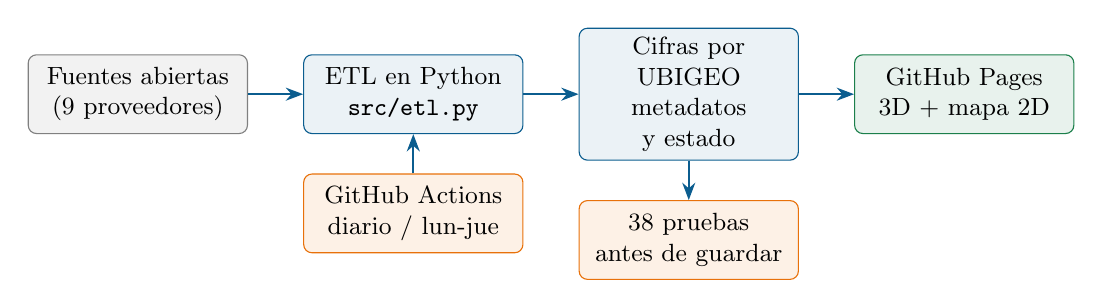
\begin{tikzpicture}[node distance=5mm and 7mm, font=\small,
  c/.style={draw=azulc, rounded corners=3pt, fill=azulc!8, align=center, minimum height=10mm, text width=2.55cm},
  f/.style={-{Stealth[length=2.2mm]}, thick, azulc}]
\node[c,fill=gray!10,draw=gray] (a) {Fuentes abiertas\\(9 proveedores)};
\node[c,right=of a] (b) {ETL en Python\\\texttt{src/etl.py}};
\node[c,right=of b] (c) {Cifras por UBIGEO\\metadatos y estado};
\node[c,right=of c,fill=ok!10,draw=ok] (d) {GitHub Pages\\3D + mapa 2D};
\node[c,below=of b,fill=naranja!10,draw=naranja] (e) {GitHub Actions\\diario / lun-jue};
\node[c,below=of c,fill=naranja!10,draw=naranja] (t) {38 pruebas\\antes de guardar};
\draw[f] (a)--(b); \draw[f] (b)--(c); \draw[f] (c)--(d); \draw[f] (e)--(b); \draw[f] (c)--(t);
\end{tikzpicture}
\vspace{4mm}
\begin{itemize}\small
\item Si una fuente falla, se \textbf{conserva el último resultado válido} y se rotula como \emph{rezagado}.
\item Cada capa declara fuente, licencia, unidades, periodo y estado: \emph{vigente}, \emph{rezagado}, \emph{no disponible} o \emph{estimado}.
\item Versiones con huella SHA-256: ningún cambio de cifra pasa en silencio.
\end{itemize}
\end{frame}

% ---------- 3 ----------
\section{Auditoría}
\begin{frame}{3. Auditoría: el hallazgo crítico}
\begin{columns}[c]
\column{0.42\textwidth}
\begin{alertblock}{La población estaba desplazada $\sim$7,9 km al oeste}
\small El recorte de WorldPop salía del borde del archivo de Perú y quedó corrido 86 columnas. La población de Castilla aparecía en Piura y la de Tumbes en Corrales.
\end{alertblock}
\small\textbf{Cómo lo probamos:} con una fuente independiente. La correlación con la densidad de edificaciones pasa de \textbf{0,00} a \textbf{0,80} al corregirlo.
\column{0.56\textwidth}
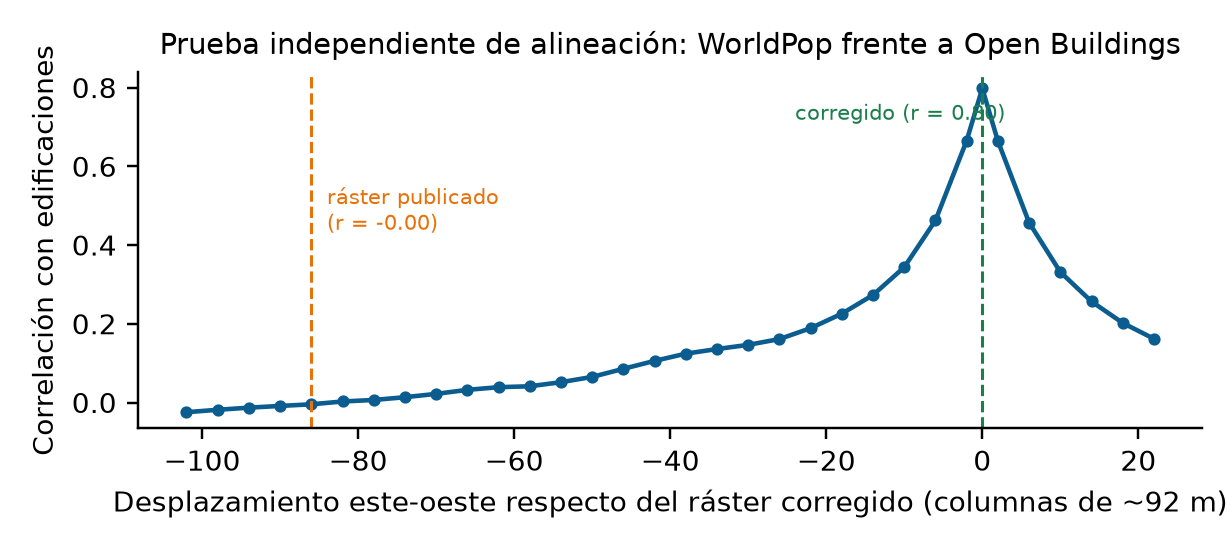
\includegraphics[width=\linewidth]{alineacion_poblacion.png}
\end{columns}
\end{frame}

\begin{frame}{3. Otras correcciones y su efecto}
\begin{columns}[T]
\column{0.44\textwidth}\small
\begin{itemize}
\item \textbf{Colegios:} «684 / 1\,268 / 684» eran anillos, no acumulados. Hasta 1 km hay \textbf{2\,636}.
\item \textbf{Sumas:} Piura + Tumbes no daba el total; faltaban \textbf{4\,138} edificaciones fuera de los polígonos.
\item \textbf{Radar reciente:} la referencia seca se solapaba con el evento. Ya está recalculado.
\item \textbf{«Viviendas»} pasan a llamarse \textbf{edificaciones} (Open Buildings detecta cualquier uso).
\item \textbf{Sin GPU:} el 3D fallaba sin WebGL; ahora hay un mapa 2D.
\end{itemize}
\column{0.54\textwidth}
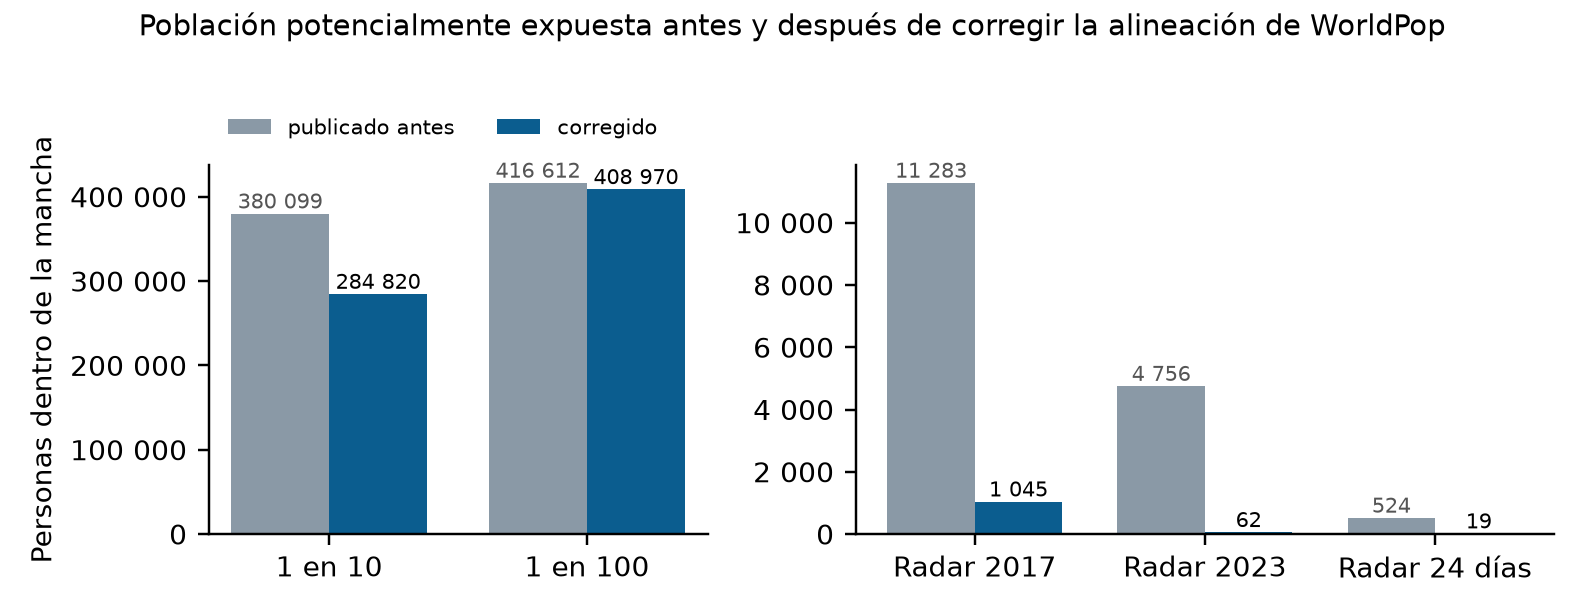
\includegraphics[width=\linewidth]{antes_despues_poblacion.png}\\
\scriptsize En 2023, la mancha (86\,\% en el desierto de Sechura) tenía 62 personas, no 4\,756.
\end{columns}
\end{frame}

% ---------- 4 ----------
\section{Resultados}
\begin{frame}{4. Resultados: zona inundable de 1 en 100 años (JRC)}
\vspace{2mm}
\centering
\cifra{3\,793 km²}{superficie inundable}\hfill
\cifra{399\,506}{personas potencialmente expuestas}\hfill
\cifra{148\,348}{edificaciones potencialmente expuestas}\hfill
\cifra{682 · 145}{locales escolares · establecimientos de salud dentro}
\vspace{6mm}
\begin{columns}[T]
\column{0.5\textwidth}
\begin{block}{Distritos más expuestos (población)}\small
Castilla 71\,184 · Catacaos 70\,167 (85\,\% de su población) · Piura 55\,762 · La Unión 29\,090 · La Arena 23\,909
\end{block}
\column{0.46\textwidth}
\begin{block}{Hasta 1 km de la mancha (acumulado)}\small
2\,633 locales escolares · 577 establecimientos de salud · 985 mil personas hasta 500 m
\end{block}
\end{columns}
\end{frame}

\begin{frame}{4. Panel de decisiones: prioridad relativa por distrito}
\begin{columns}[c]
\column{0.40\textwidth}
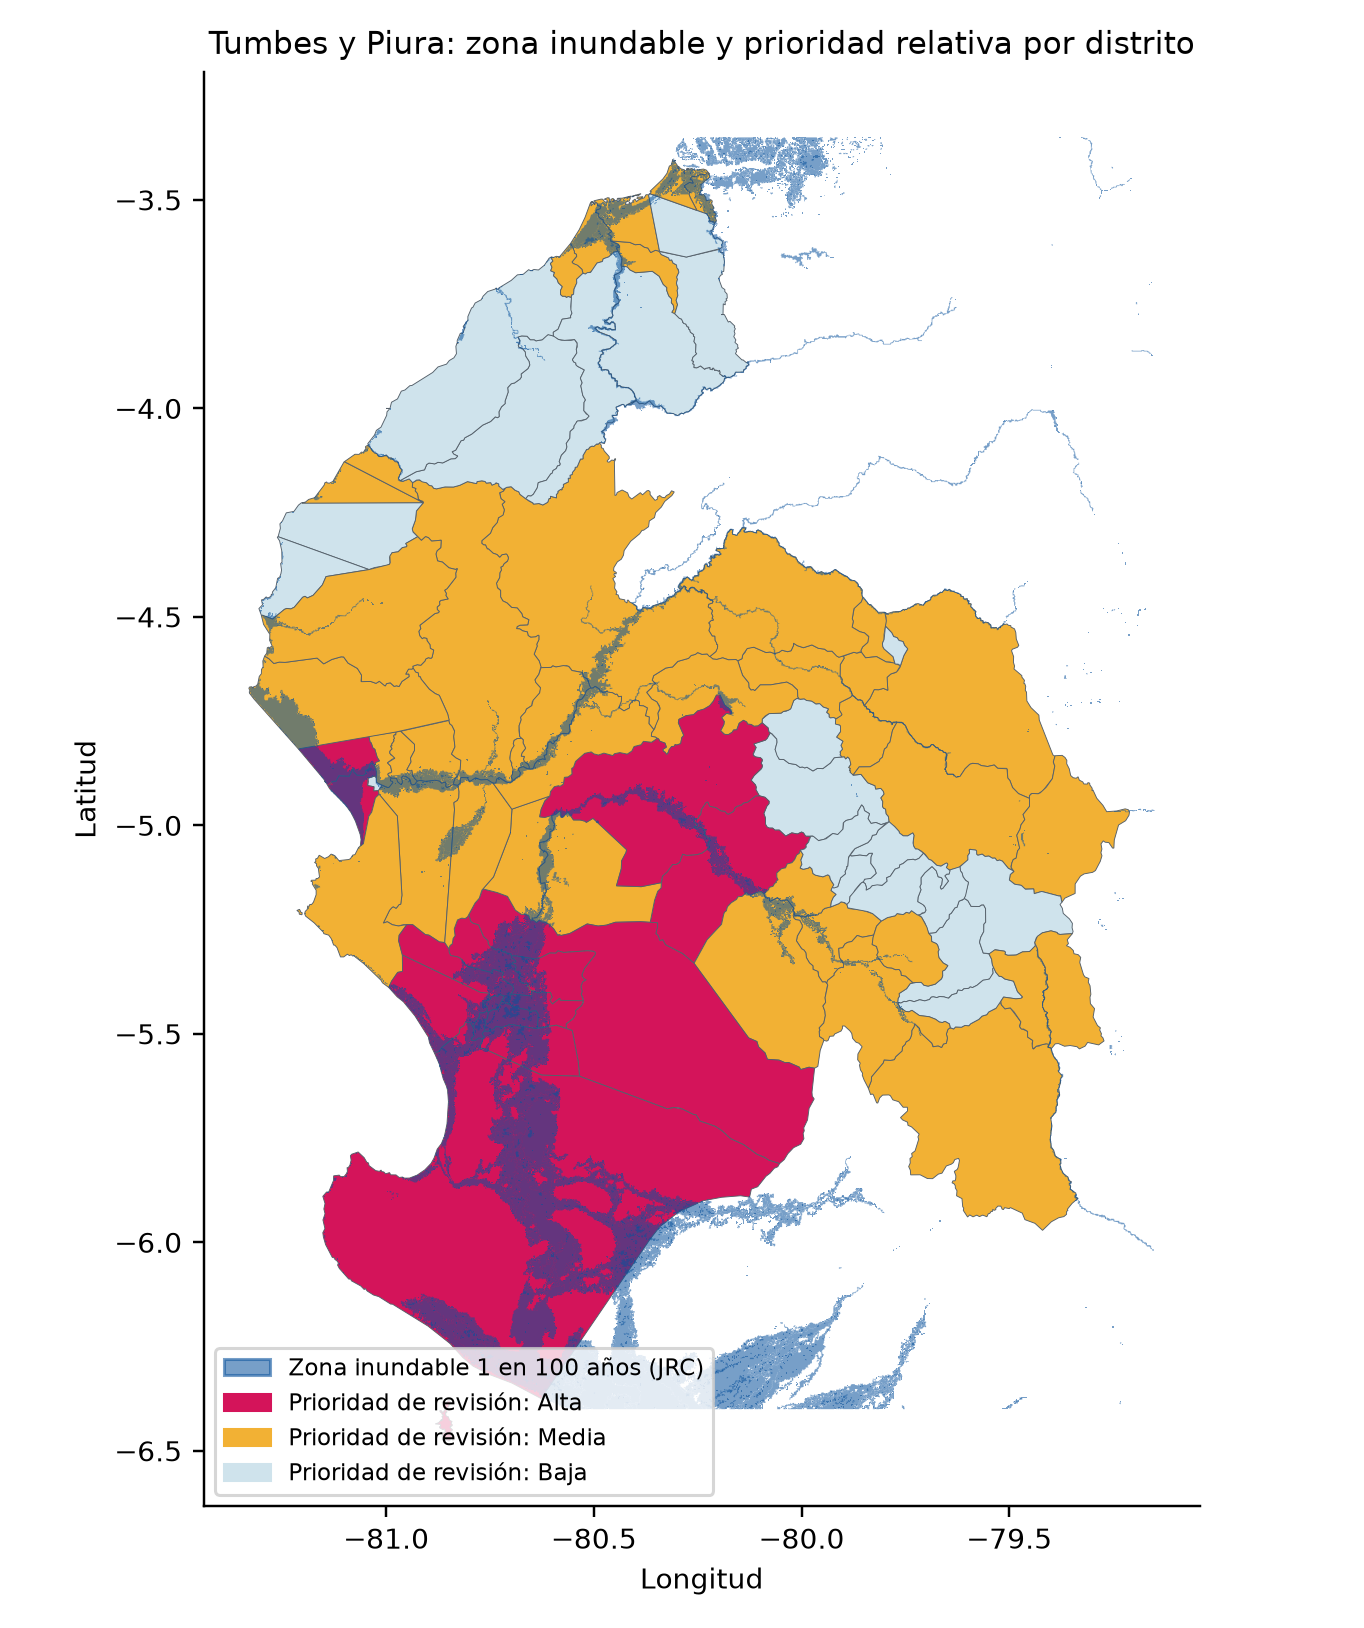
\includegraphics[height=0.82\textheight]{mapa_prioridad.png}
\column{0.58\textwidth}\small
Cuatro dimensiones \textbf{separadas}:
\begin{itemize}
\item \textbf{Peligro:} \% del distrito en la zona 1/100
\item \textbf{Exposición:} población dentro
\item \textbf{Vulnerabilidad:} pobreza monetaria 2018
\item \textbf{Riesgo estimado:} promedio de percentiles (0--100)
\end{itemize}
\vspace{2mm}
\textbf{Prioridad alta (15 de 76):} La Arena, Bernal, La Unión, El Tallán, Colán, Cura Mori, Catacaos, Tambo Grande, Chulucanas…
\vspace{2mm}

\scriptsize\color{gris} Es un orden relativo para priorizar revisiones; no reemplaza las evaluaciones oficiales (EVAR/CENEPRED).
\end{columns}
\end{frame}

% ---------- 5 ----------
\section{Tablero}
\begin{frame}{5. El tablero publicado: mapa 2D accesible}
\centering
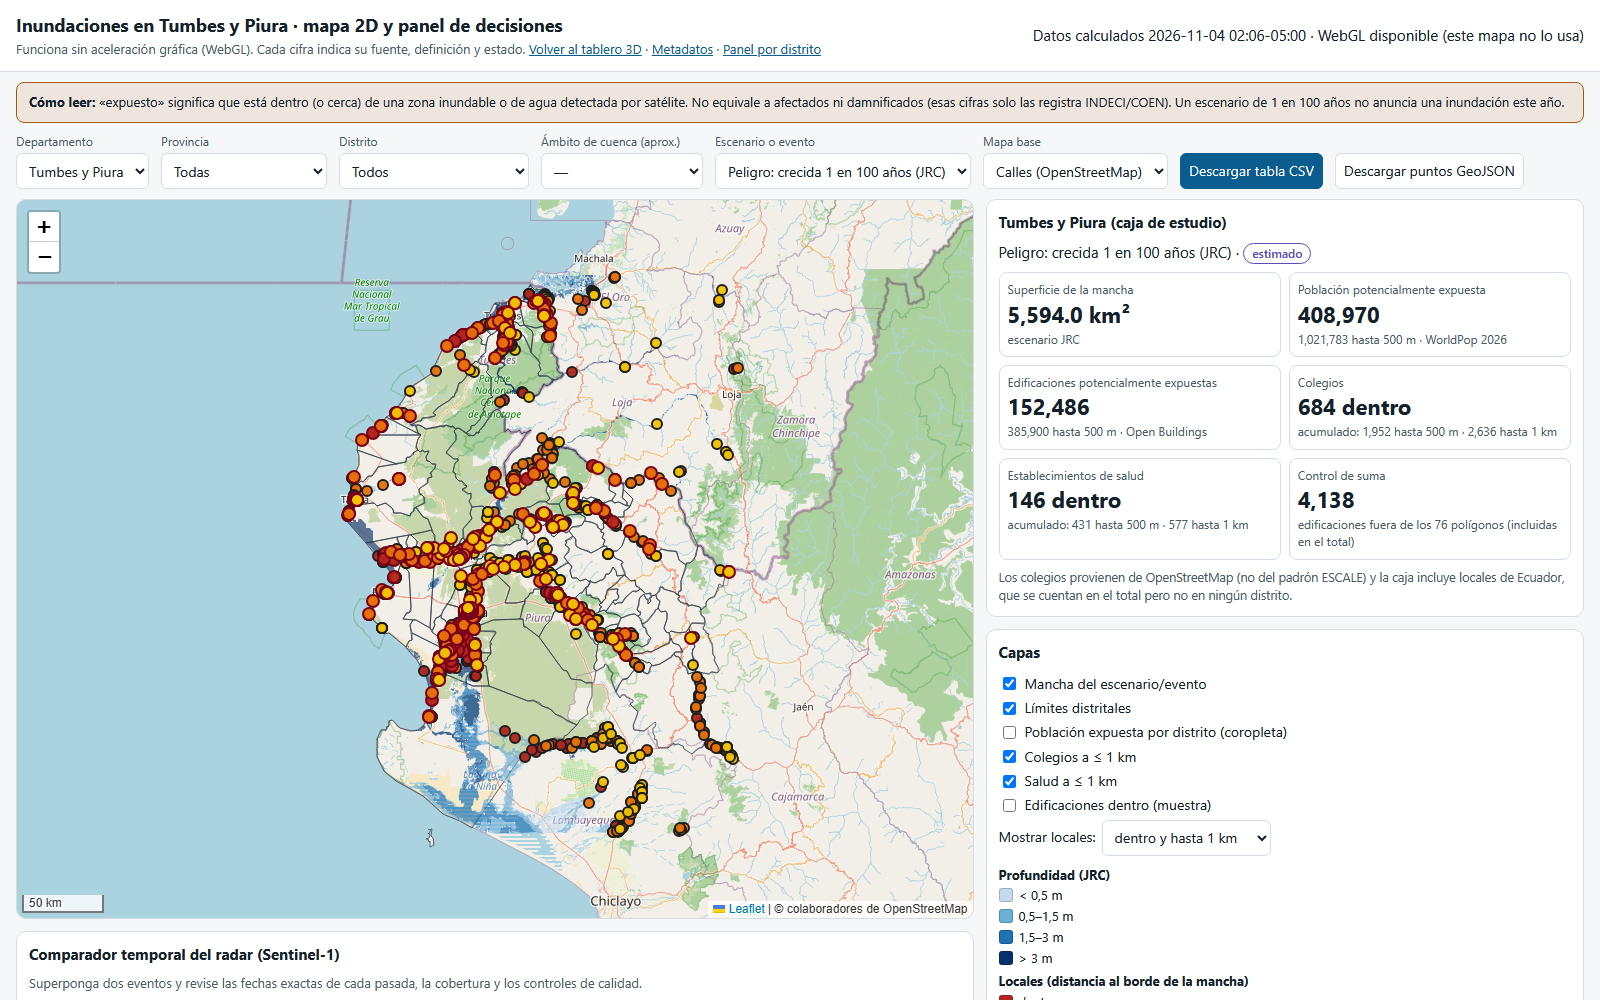
\includegraphics[height=0.76\textheight]{captura_mapa2d.png}\\
\scriptsize Selector de departamento, provincia, distrito y cuenca · 5 escenarios · comparador del radar · metadatos · descargas CSV/GeoJSON · funciona en celular y sin GPU
\end{frame}

% ---------- 6 ----------
\section{Validación}
\begin{frame}{6. ¿Funcionó en Tumbes y Piura? Validación externa con INDECI}
\begin{columns}[c]
\column{0.60\textwidth}
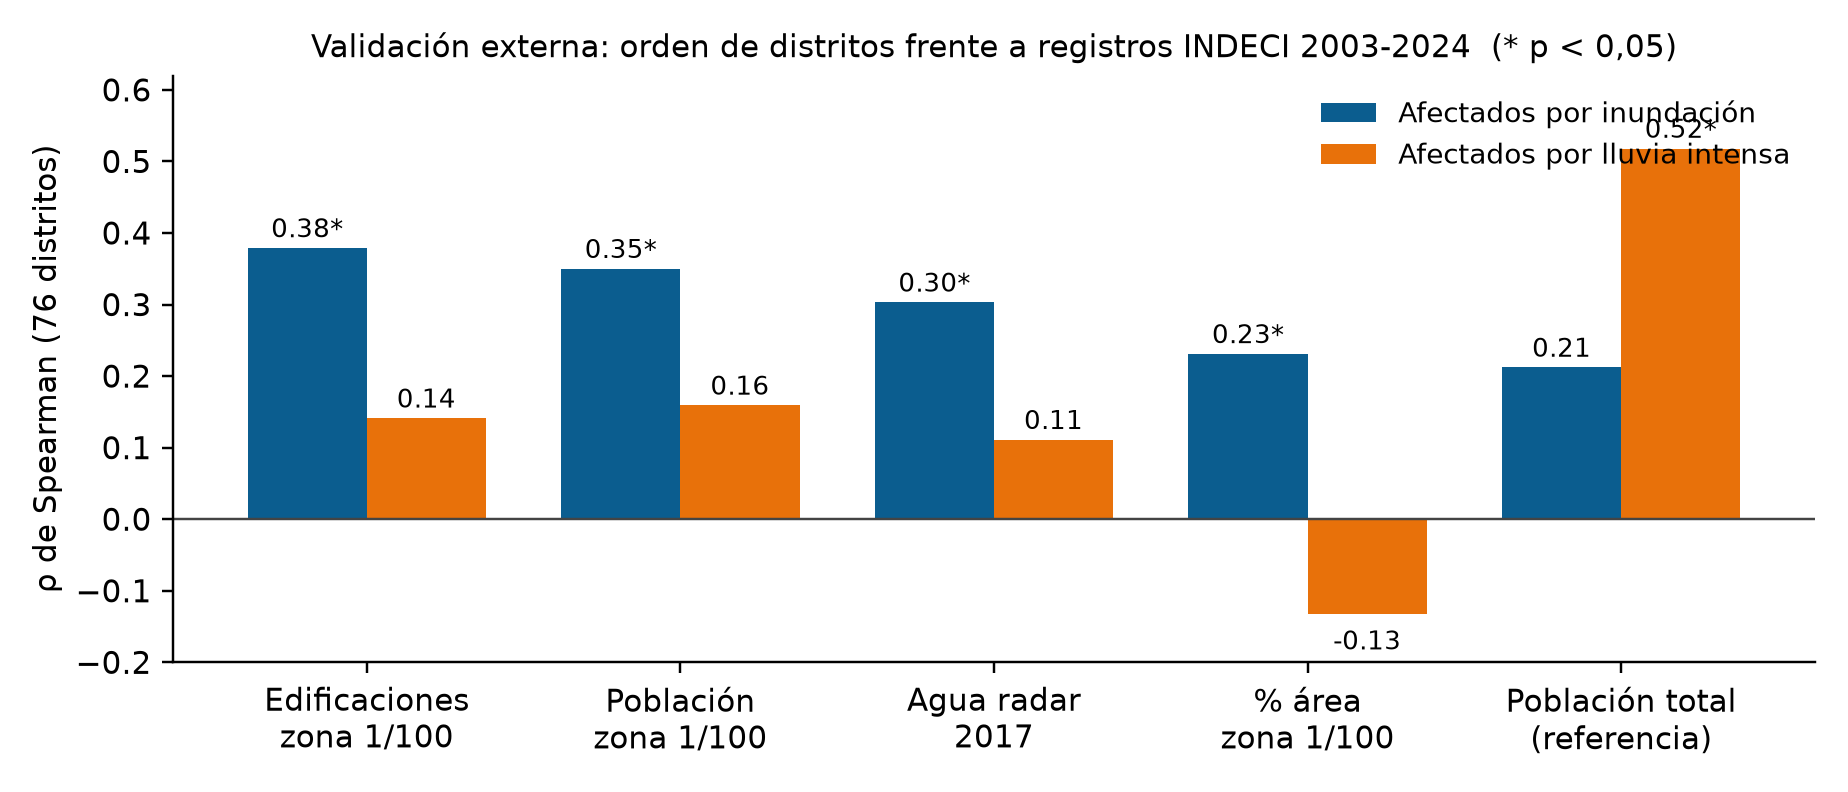
\includegraphics[width=\linewidth]{validacion_indeci.png}
\column{0.38\textwidth}\small
\begin{exampleblock}{Inundación por desborde: sí}
La exposición ordena los distritos como los afectados por inundación de INDECI ($\rho$ = 0,38, p < 0,001), mejor que la población total (0,21). Coinciden \textbf{9 de 15} distritos del top.
\end{exampleblock}
\begin{alertblock}{Lluvia intensa: no}
Los daños por lluvia y huaicos (zonas altas) los explica la población, no la zona inundable fluvial.
\end{alertblock}
\end{columns}
\end{frame}

\begin{frame}{6. Lo que todavía no funciona bien}
\begin{columns}[T]
\column{0.5\textwidth}
\begin{alertblock}{Radar en ciudades}\small
Catacaos 2017: solo 1,1 km² detectados, aunque fue de los distritos más inundados. El radar con umbral fijo sirve como \textbf{mínimo}, no como verdad-terreno.
\end{alertblock}
\begin{alertblock}{Datos base}\small
Faltan 2 distritos en los límites (Veintiséis de Octubre y Canoas de Punta Sal); los colegios no vienen del padrón oficial ESCALE; no hay daños fechados después de 2015.
\end{alertblock}
\column{0.46\textwidth}
\begin{block}{Capa de radar reciente (recalculada)}\small
13 pasadas del 12/10 al 2/11/2026; referencia seca con 42 pasadas.\\
\textbf{27,2 km²} de agua nueva en tierra (77\,\% en Sechura): 24 personas y 8 edificaciones dentro.\\
Umbral Otsu automático: $-16{,}8$ dB, frente al fijo de $-17$ dB.\\
En temporada seca: es sobre todo riego y humedales.
\end{block}
\end{columns}
\end{frame}

% ---------- 7 ----------
\section{Machine learning}
\begin{frame}{7. Machine learning: experimentar sin inventar exactitud}
\begin{columns}[c]
\column{0.55\textwidth}
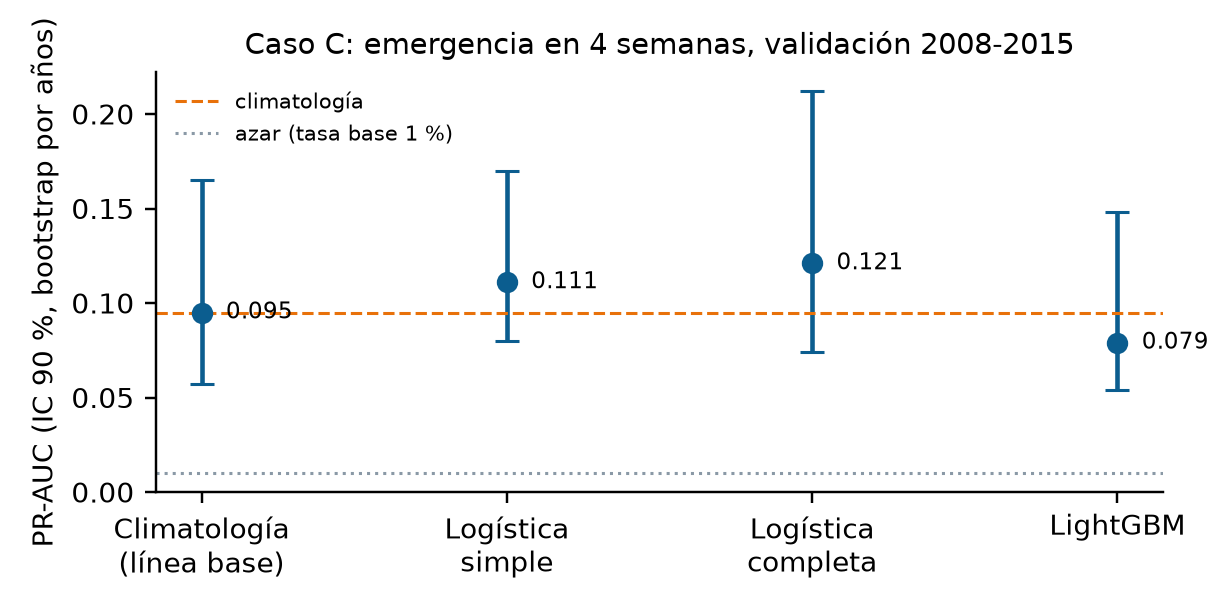
\includegraphics[width=\linewidth]{ml_pr_auc.png}
\column{0.43\textwidth}\small
\textbf{Caso C:} ¿habrá una emergencia en el distrito en 4 semanas? Validación por años (2008--2015), con 311 casos.
\begin{itemize}
\item La logística simple supera a la climatología con probabilidad 0,92, pero el IC de la diferencia \textbf{incluye el 0}.
\item LightGBM no mejora la línea base.
\item Captura el 46\,\% de las emergencias de Tumbes y solo el \textbf{5\,\%} de las de Piura.
\end{itemize}
\textbf{Casos A y B} (susceptibilidad y SAR): no entrenamos porque \textbf{no hay etiquetas independientes}.
\end{columns}
\end{frame}

% ---------- 8 ----------
\section{Aporte}
\begin{frame}{8. Aporte al INEI y políticas públicas}
\begin{columns}[T]
\column{0.48\textwidth}
\begin{block}{Aporte estadístico (el INEI produce estadística, no alertas)}\small
\textbf{Indicador:} población y edificaciones potencialmente expuestas a la zona 1/100 \textbf{por UBIGEO}, con metadatos, diccionario de variables y periodicidad anual. Interoperable con CENEPRED, MINEDU, MINSA, ANA y SENAMHI.
\end{block}
\column{0.48\textwidth}
\begin{block}{7 opciones de política (para evaluar)}\small
\begin{enumerate}
\item Continuidad educativa (682 locales escolares dentro, 124\,385 alumnos)
\item Continuidad de los servicios de salud (145 dentro)
\item Ordenamiento territorial
\item Mantenimiento focalizado de drenes
\item Rutas de evacuación y refugios
\item Comunicación de riesgo
\item Levantamiento de datos
\end{enumerate}
\end{block}
\end{columns}
\end{frame}

% ---------- 9 ----------
\section{Expansión}
\begin{frame}{9. ¿Se puede expandir? Escala con los costos medidos}
\begin{columns}[c]
\column{0.66\textwidth}\scriptsize
\begin{tabularx}{\linewidth}{>{\raggedright\arraybackslash}Xp{0.7cm}p{1.1cm}p{0.8cm}p{1.4cm}}\toprule
\textbf{Escenario} & \textbf{Dist.} & \textbf{Población} & \textbf{Área} & \textbf{Radar/evento}\\\midrule
Piloto: Tumbes, Piura & 78 & 2,3 M & 1× & $\sim$40 min\\
\textbf{Norte costero} (+ Lambayeque, La Libertad) & 199 & 5,8 M & 3,6× & $\sim$2,4 h\\
Norte ampliado (+ Cajamarca, Áncash) & 492 & 8,6 M & 4,9× & $\sim$3,3 h\\
Perú & 1\,893 & 34,4 M & 33,5× & $\sim$22 h\\\bottomrule
\end{tabularx}
\vspace{3mm}
\begin{itemize}\footnotesize
\item \textbf{Norte costero: viable a corto plazo}, procesando por departamento (1--2 semanas de trabajo).
\item \textbf{Sierra norte:} hace falta otra capa de peligro (lluvia, huaicos: CENEPRED, INGEMMET).
\item \textbf{Perú:} posible si se reorganiza por departamento, con teselas, el radar solo por evento y otra lógica para la Amazonía.
\end{itemize}
\column{0.31\textwidth}
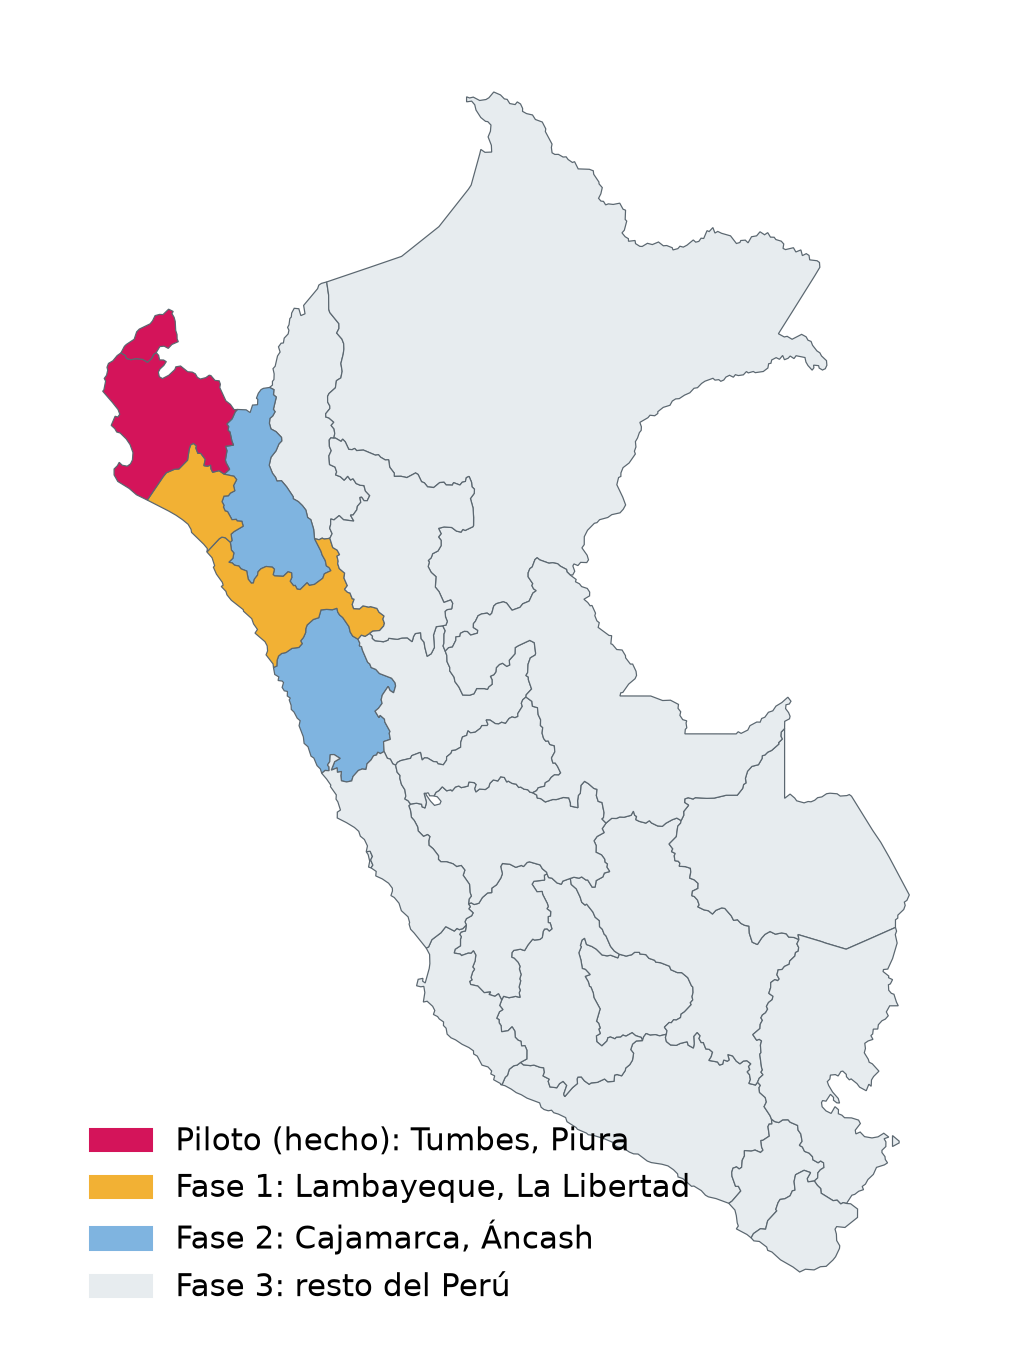
\includegraphics[width=\linewidth]{fases_expansion.png}
\end{columns}
\end{frame}

% ---------- 10 ----------
\section{Próximos pasos}
\begin{frame}{10. Propuesta para consultar con el docente}
\begin{columns}[T]
\column{0.5\textwidth}
\begin{block}{Corto plazo (P0--P1)}\footnotesize
\begin{itemize}
\item Límites oficiales del INEI (78 distritos) y padrón ESCALE
\item Validar la población con el Censo 2017 y las proyecciones del INEI
\item Agregar una capa de lluvia intensa y huaicos (la carencia detectada)
\end{itemize}
\end{block}
\begin{block}{Mediano plazo (P2)}\footnotesize
\begin{itemize}
\item Referencia independiente de inundación 2017/2023 para validar el radar
\item Susceptibilidad espacial (HAND, uso del suelo) con validación por cuenca
\end{itemize}
\end{block}
\column{0.46\textwidth}
\begin{exampleblock}{Pregunta al docente}\small
¿Ampliamos a la \textbf{costa norte} (4 departamentos) para mostrar que el método se transfiere, o profundizamos primero la validación en Tumbes y Piura?
\end{exampleblock}
\vspace{2mm}
\small\textbf{Evidencia reproducible}
\begin{itemize}\footnotesize
\item \texttt{python src/etl.py local}
\item \texttt{python -m pytest} (38 pruebas)
\item Documentos 01--06 e informe en Word
\end{itemize}
\end{columns}
\end{frame}

{\setbeamertemplate{footline}{}
\begin{frame}
\begin{tikzpicture}[remember picture,overlay]
\fill[azul] (current page.south west) rectangle (current page.north east);
\node[text=white,align=center] at (current page.center) {{\huge\bfseries Gracias}\\[10pt]
  \large Tablero: \texttt{marciashapiama.github.io/iapn-inei}\\[3pt]
  Mapa 2D: \texttt{marciashapiama.github.io/iapn-inei/mapa2d.html}\\[3pt]
  Código y documentos: \texttt{github.com/MarciaShapiama/iapn-inei}};
\end{tikzpicture}
\end{frame}}

\end{document}
